%% LyX 1.1 created this file.  For more info, see http://www.lyx.org/.
%% Do not edit unless you really know what you are doing.
\documentclass[german]{slides}
\usepackage[T1]{fontenc}
\usepackage{babel}
\usepackage[dvips]{graphics}

\makeatletter


%%%%%%%%%%%%%%%%%%%%%%%%%%%%%% LyX specific LaTeX commands.
\providecommand{\LyX}{L\kern-.1667em\lower.25em\hbox{Y}\kern-.125emX\@}

%%%%%%%%%%%%%%%%%%%%%%%%%%%%%% Textclass specific LaTeX commands.
 \newcounter{slidetype}
 \setcounter{slidetype}{0}
 \newif\ifLyXsNoCenter
 \LyXsNoCenterfalse
 \newcommand{\noslidecentering}{
    \LyXsNoCentertrue%
 }
 \newcommand{\slidecentering}{
    \LyXsNoCenterfalse%
 }
 \newcommand{\lyxendslide}[1]{
    \ifLyXsNoCenter%
         \vfill%
    \fi%
    \ifcase \value{slidetype}%
         \or % no action for 0
         \end{slide} \or%
         \end{overlay} \or%
         \end{note}%
    \fi%
    \setcounter{slidetype}{0}
	\visible
 }
 \AtEndDocument{\lyxendslide{.}}
 \newcommand{\lyxnewslide}[1]{
    \lyxendslide{.}
    \setcounter{slidetype}{1}
    \begin{slide}
 }
 \newenvironment{lyxcode}
   {\begin{list}{}{
     \setlength{\rightmargin}{\leftmargin}
     \raggedright
     \setlength{\itemsep}{0pt}
     \setlength{\parsep}{0pt}
     \verbatim@font}%
    \item[]}
   {\end{list}}

%%%%%%%%%%%%%%%%%%%%%%%%%%%%%% User specified LaTeX commands.
% Uncomment to print out only slides and overlays
%
%\onlyslides{\slides}

% Uncomment to print out only notes
%
%\onlynotes{\notes}

\usepackage{textcomp}
\makeatother

\begin{document}


\lyxnewslide{}

{\par\centering \textbf{\Large Werkzeugunterst�tzung f�r die �berpr�fung der
Einhaltung von OCL-Gesch�ftsregeln in Java-Programmen}\Large \par}

{\par\centering Ralf Wiebicke\par}

{\par\centering 6. Februar 2001\par}


\lyxnewslide{}

{\par\centering \textbf{\Large �bersicht}\Large \par}

\vspace{10pt}\hrule height 4pt

\begin{itemize}
\item Vorstellung der Arbeit
\item Stellungnahme Gutachten
\item Zusammenfassung
\end{itemize}

\lyxnewslide{}

{\par\centering \textbf{\Large Kritikpunkte der Gutachten}\Large \par}

\vspace{10pt}\hrule height 4pt

\begin{itemize}
\item Dokumentation der Experimente mit dem Industriebeispiel

\begin{itemize}
\item Dokumentation in anderen Kapiteln
\item hoher Aufwand bis zur Lauff�higkeit
\item Verzicht auf die Dokumentation des \\
net-linx-Modells
\end{itemize}
\item geringe Abstraktion
\item Injektivit�t der Hashfunktion
\item Integration mit UML-CASE-Tools
\end{itemize}

\lyxnewslide{}

{\par\centering \textbf{\Large Constraints des Industriebeispiels}\Large \par}

\vspace{10pt}\hrule height 4pt

\vspace{0cm}
{\par\centering \resizebox*{1\textwidth}{!}{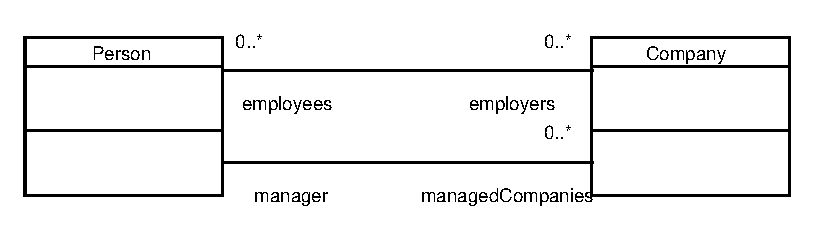
\includegraphics{PersonCompany.eps}} \par}
\vspace{0cm}

\begin{lyxcode}
context~Person~inv:

~~employers->forAll(

~~~~employees->includes(self))

~

context~Person~inv:

~~isMarried~implies~

~~~~(wife->isEmpty~xor~husband->isEmpty)

~

context~Company~inv:~employees->size>0

~

context~Company~inv:~

~~uppername=name.toUpper
\end{lyxcode}

\lyxnewslide{}

{\par\centering \textbf{\Large Vererbung von Vorbedingungen}\Large \par}

\vspace{10pt}\hrule height 4pt

\begin{lyxcode}
context~Super::method()

~~pre:~a

~~pre:~b

~

context~Sub::method()

~~pre:~a'
\end{lyxcode}
\vspace{10pt}\hrule height 2pt

\begin{lyxcode}
context~Konto::abheben(betrag)

~~pre:~guthaben-betrag>=0

~~pre:~betrag<=10000

~

context~DispoKonto::abheben(betrag)

~~pre:~guthaben-betrag>=(-1000)
\end{lyxcode}

\lyxnewslide{}

{\par\centering \textbf{\Large Zusammenfassung}\Large \par}

\vspace{10pt}\hrule height 4pt

\begin{itemize}
\item erprobte Implementation
\item Javaparser auf Signaturlevel
\item Caching von Invarianten
\item Typinformation f�r Java Collections
\item Reversible Codeinstrumentation
\item Einf�geschema ``Method Wrappers''
\end{itemize}
\end{document}
